\begin{figure}[htbp]
\centering
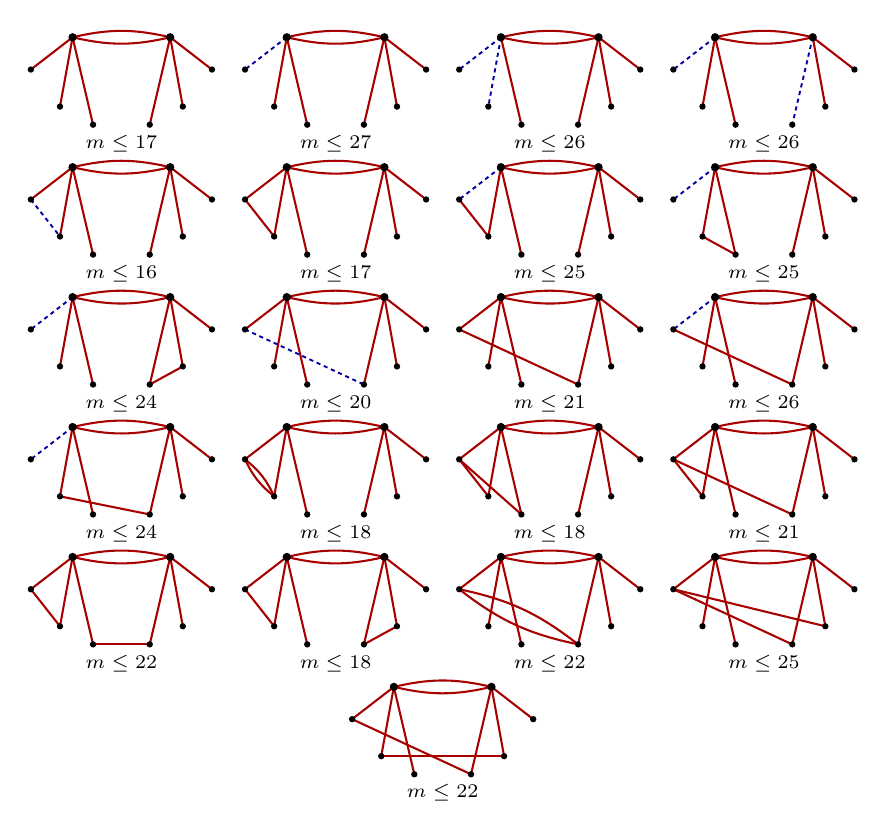
\begin{tikzpicture}[font=\scriptsize,
sc marked/.style={draw=red!65!black,line width=.75pt},
sc unmarked/.style={draw=blue!65!black,line width=.68pt,dash pattern=on 1.5pt off 1.35pt}]
\begin{scope}[shift={(-4.08,0)}]
\coordinate (u) at (-0.62,0.35);
\coordinate (v) at (0.62,0.35);
\coordinate (a0) at (-1.15,-0.06);
\coordinate (a1) at (-0.78,-0.53);
\coordinate (a2) at (-0.36,-0.76);
\coordinate (a3) at (0.36,-0.76);
\coordinate (a4) at (0.78,-0.53);
\coordinate (a5) at (1.15,-0.06);
\draw[sc marked] (u) to[bend left=13] (v);
\draw[sc marked] (u) to[bend right=13] (v);
\draw[sc marked] (u) -- (a0);
\draw[sc marked] (u) -- (a1);
\draw[sc marked] (u) -- (a2);
\draw[sc marked] (v) -- (a3);
\draw[sc marked] (v) -- (a4);
\draw[sc marked] (v) -- (a5);
\fill (u) circle[radius=1.5pt];
\fill (v) circle[radius=1.5pt];
\fill (a0) circle[radius=1.15pt];
\fill (a1) circle[radius=1.15pt];
\fill (a2) circle[radius=1.15pt];
\fill (a3) circle[radius=1.15pt];
\fill (a4) circle[radius=1.15pt];
\fill (a5) circle[radius=1.15pt];
\node[anchor=north,inner sep=1pt] at (0,-.85) {\(m\leq 17\)};
\end{scope}
\begin{scope}[shift={(-1.36,0)}]
\coordinate (u) at (-0.62,0.35);
\coordinate (v) at (0.62,0.35);
\coordinate (a0) at (-1.15,-0.06);
\coordinate (a1) at (-0.78,-0.53);
\coordinate (a2) at (-0.36,-0.76);
\coordinate (a3) at (0.36,-0.76);
\coordinate (a4) at (0.78,-0.53);
\coordinate (a5) at (1.15,-0.06);
\draw[sc marked] (u) to[bend left=13] (v);
\draw[sc marked] (u) to[bend right=13] (v);
\draw[sc unmarked] (u) -- (a0);
\draw[sc marked] (u) -- (a1);
\draw[sc marked] (u) -- (a2);
\draw[sc marked] (v) -- (a3);
\draw[sc marked] (v) -- (a4);
\draw[sc marked] (v) -- (a5);
\fill (u) circle[radius=1.5pt];
\fill (v) circle[radius=1.5pt];
\fill (a0) circle[radius=1.15pt];
\fill (a1) circle[radius=1.15pt];
\fill (a2) circle[radius=1.15pt];
\fill (a3) circle[radius=1.15pt];
\fill (a4) circle[radius=1.15pt];
\fill (a5) circle[radius=1.15pt];
\node[anchor=north,inner sep=1pt] at (0,-.85) {\(m\leq 27\)};
\end{scope}
\begin{scope}[shift={(1.36,0)}]
\coordinate (u) at (-0.62,0.35);
\coordinate (v) at (0.62,0.35);
\coordinate (a0) at (-1.15,-0.06);
\coordinate (a1) at (-0.78,-0.53);
\coordinate (a2) at (-0.36,-0.76);
\coordinate (a3) at (0.36,-0.76);
\coordinate (a4) at (0.78,-0.53);
\coordinate (a5) at (1.15,-0.06);
\draw[sc marked] (u) to[bend left=13] (v);
\draw[sc marked] (u) to[bend right=13] (v);
\draw[sc unmarked] (u) -- (a0);
\draw[sc unmarked] (u) -- (a1);
\draw[sc marked] (u) -- (a2);
\draw[sc marked] (v) -- (a3);
\draw[sc marked] (v) -- (a4);
\draw[sc marked] (v) -- (a5);
\fill (u) circle[radius=1.5pt];
\fill (v) circle[radius=1.5pt];
\fill (a0) circle[radius=1.15pt];
\fill (a1) circle[radius=1.15pt];
\fill (a2) circle[radius=1.15pt];
\fill (a3) circle[radius=1.15pt];
\fill (a4) circle[radius=1.15pt];
\fill (a5) circle[radius=1.15pt];
\node[anchor=north,inner sep=1pt] at (0,-.85) {\(m\leq 26\)};
\end{scope}
\begin{scope}[shift={(4.08,0)}]
\coordinate (u) at (-0.62,0.35);
\coordinate (v) at (0.62,0.35);
\coordinate (a0) at (-1.15,-0.06);
\coordinate (a1) at (-0.78,-0.53);
\coordinate (a2) at (-0.36,-0.76);
\coordinate (a3) at (0.36,-0.76);
\coordinate (a4) at (0.78,-0.53);
\coordinate (a5) at (1.15,-0.06);
\draw[sc marked] (u) to[bend left=13] (v);
\draw[sc marked] (u) to[bend right=13] (v);
\draw[sc unmarked] (u) -- (a0);
\draw[sc marked] (u) -- (a1);
\draw[sc marked] (u) -- (a2);
\draw[sc unmarked] (v) -- (a3);
\draw[sc marked] (v) -- (a4);
\draw[sc marked] (v) -- (a5);
\fill (u) circle[radius=1.5pt];
\fill (v) circle[radius=1.5pt];
\fill (a0) circle[radius=1.15pt];
\fill (a1) circle[radius=1.15pt];
\fill (a2) circle[radius=1.15pt];
\fill (a3) circle[radius=1.15pt];
\fill (a4) circle[radius=1.15pt];
\fill (a5) circle[radius=1.15pt];
\node[anchor=north,inner sep=1pt] at (0,-.85) {\(m\leq 26\)};
\end{scope}
\begin{scope}[shift={(-4.08,-1.65)}]
\coordinate (u) at (-0.62,0.35);
\coordinate (v) at (0.62,0.35);
\coordinate (a0) at (-1.15,-0.06);
\coordinate (a1) at (-0.78,-0.53);
\coordinate (a2) at (-0.36,-0.76);
\coordinate (a3) at (0.36,-0.76);
\coordinate (a4) at (0.78,-0.53);
\coordinate (a5) at (1.15,-0.06);
\draw[sc marked] (u) to[bend left=13] (v);
\draw[sc marked] (u) to[bend right=13] (v);
\draw[sc marked] (u) -- (a0);
\draw[sc marked] (u) -- (a1);
\draw[sc marked] (u) -- (a2);
\draw[sc marked] (v) -- (a3);
\draw[sc marked] (v) -- (a4);
\draw[sc marked] (v) -- (a5);
\draw[sc unmarked] (a0) -- (a1);
\fill (u) circle[radius=1.5pt];
\fill (v) circle[radius=1.5pt];
\fill (a0) circle[radius=1.15pt];
\fill (a1) circle[radius=1.15pt];
\fill (a2) circle[radius=1.15pt];
\fill (a3) circle[radius=1.15pt];
\fill (a4) circle[radius=1.15pt];
\fill (a5) circle[radius=1.15pt];
\node[anchor=north,inner sep=1pt] at (0,-.85) {\(m\leq 16\)};
\end{scope}
\begin{scope}[shift={(-1.36,-1.65)}]
\coordinate (u) at (-0.62,0.35);
\coordinate (v) at (0.62,0.35);
\coordinate (a0) at (-1.15,-0.06);
\coordinate (a1) at (-0.78,-0.53);
\coordinate (a2) at (-0.36,-0.76);
\coordinate (a3) at (0.36,-0.76);
\coordinate (a4) at (0.78,-0.53);
\coordinate (a5) at (1.15,-0.06);
\draw[sc marked] (u) to[bend left=13] (v);
\draw[sc marked] (u) to[bend right=13] (v);
\draw[sc marked] (u) -- (a0);
\draw[sc marked] (u) -- (a1);
\draw[sc marked] (u) -- (a2);
\draw[sc marked] (v) -- (a3);
\draw[sc marked] (v) -- (a4);
\draw[sc marked] (v) -- (a5);
\draw[sc marked] (a0) -- (a1);
\fill (u) circle[radius=1.5pt];
\fill (v) circle[radius=1.5pt];
\fill (a0) circle[radius=1.15pt];
\fill (a1) circle[radius=1.15pt];
\fill (a2) circle[radius=1.15pt];
\fill (a3) circle[radius=1.15pt];
\fill (a4) circle[radius=1.15pt];
\fill (a5) circle[radius=1.15pt];
\node[anchor=north,inner sep=1pt] at (0,-.85) {\(m\leq 17\)};
\end{scope}
\begin{scope}[shift={(1.36,-1.65)}]
\coordinate (u) at (-0.62,0.35);
\coordinate (v) at (0.62,0.35);
\coordinate (a0) at (-1.15,-0.06);
\coordinate (a1) at (-0.78,-0.53);
\coordinate (a2) at (-0.36,-0.76);
\coordinate (a3) at (0.36,-0.76);
\coordinate (a4) at (0.78,-0.53);
\coordinate (a5) at (1.15,-0.06);
\draw[sc marked] (u) to[bend left=13] (v);
\draw[sc marked] (u) to[bend right=13] (v);
\draw[sc unmarked] (u) -- (a0);
\draw[sc marked] (u) -- (a1);
\draw[sc marked] (u) -- (a2);
\draw[sc marked] (v) -- (a3);
\draw[sc marked] (v) -- (a4);
\draw[sc marked] (v) -- (a5);
\draw[sc marked] (a0) -- (a1);
\fill (u) circle[radius=1.5pt];
\fill (v) circle[radius=1.5pt];
\fill (a0) circle[radius=1.15pt];
\fill (a1) circle[radius=1.15pt];
\fill (a2) circle[radius=1.15pt];
\fill (a3) circle[radius=1.15pt];
\fill (a4) circle[radius=1.15pt];
\fill (a5) circle[radius=1.15pt];
\node[anchor=north,inner sep=1pt] at (0,-.85) {\(m\leq 25\)};
\end{scope}
\begin{scope}[shift={(4.08,-1.65)}]
\coordinate (u) at (-0.62,0.35);
\coordinate (v) at (0.62,0.35);
\coordinate (a0) at (-1.15,-0.06);
\coordinate (a1) at (-0.78,-0.53);
\coordinate (a2) at (-0.36,-0.76);
\coordinate (a3) at (0.36,-0.76);
\coordinate (a4) at (0.78,-0.53);
\coordinate (a5) at (1.15,-0.06);
\draw[sc marked] (u) to[bend left=13] (v);
\draw[sc marked] (u) to[bend right=13] (v);
\draw[sc unmarked] (u) -- (a0);
\draw[sc marked] (u) -- (a1);
\draw[sc marked] (u) -- (a2);
\draw[sc marked] (v) -- (a3);
\draw[sc marked] (v) -- (a4);
\draw[sc marked] (v) -- (a5);
\draw[sc marked] (a1) -- (a2);
\fill (u) circle[radius=1.5pt];
\fill (v) circle[radius=1.5pt];
\fill (a0) circle[radius=1.15pt];
\fill (a1) circle[radius=1.15pt];
\fill (a2) circle[radius=1.15pt];
\fill (a3) circle[radius=1.15pt];
\fill (a4) circle[radius=1.15pt];
\fill (a5) circle[radius=1.15pt];
\node[anchor=north,inner sep=1pt] at (0,-.85) {\(m\leq 25\)};
\end{scope}
\begin{scope}[shift={(-4.08,-3.3)}]
\coordinate (u) at (-0.62,0.35);
\coordinate (v) at (0.62,0.35);
\coordinate (a0) at (-1.15,-0.06);
\coordinate (a1) at (-0.78,-0.53);
\coordinate (a2) at (-0.36,-0.76);
\coordinate (a3) at (0.36,-0.76);
\coordinate (a4) at (0.78,-0.53);
\coordinate (a5) at (1.15,-0.06);
\draw[sc marked] (u) to[bend left=13] (v);
\draw[sc marked] (u) to[bend right=13] (v);
\draw[sc unmarked] (u) -- (a0);
\draw[sc marked] (u) -- (a1);
\draw[sc marked] (u) -- (a2);
\draw[sc marked] (v) -- (a3);
\draw[sc marked] (v) -- (a4);
\draw[sc marked] (v) -- (a5);
\draw[sc marked] (a3) -- (a4);
\fill (u) circle[radius=1.5pt];
\fill (v) circle[radius=1.5pt];
\fill (a0) circle[radius=1.15pt];
\fill (a1) circle[radius=1.15pt];
\fill (a2) circle[radius=1.15pt];
\fill (a3) circle[radius=1.15pt];
\fill (a4) circle[radius=1.15pt];
\fill (a5) circle[radius=1.15pt];
\node[anchor=north,inner sep=1pt] at (0,-.85) {\(m\leq 24\)};
\end{scope}
\begin{scope}[shift={(-1.36,-3.3)}]
\coordinate (u) at (-0.62,0.35);
\coordinate (v) at (0.62,0.35);
\coordinate (a0) at (-1.15,-0.06);
\coordinate (a1) at (-0.78,-0.53);
\coordinate (a2) at (-0.36,-0.76);
\coordinate (a3) at (0.36,-0.76);
\coordinate (a4) at (0.78,-0.53);
\coordinate (a5) at (1.15,-0.06);
\draw[sc marked] (u) to[bend left=13] (v);
\draw[sc marked] (u) to[bend right=13] (v);
\draw[sc marked] (u) -- (a0);
\draw[sc marked] (u) -- (a1);
\draw[sc marked] (u) -- (a2);
\draw[sc marked] (v) -- (a3);
\draw[sc marked] (v) -- (a4);
\draw[sc marked] (v) -- (a5);
\draw[sc unmarked] (a0) -- (a3);
\fill (u) circle[radius=1.5pt];
\fill (v) circle[radius=1.5pt];
\fill (a0) circle[radius=1.15pt];
\fill (a1) circle[radius=1.15pt];
\fill (a2) circle[radius=1.15pt];
\fill (a3) circle[radius=1.15pt];
\fill (a4) circle[radius=1.15pt];
\fill (a5) circle[radius=1.15pt];
\node[anchor=north,inner sep=1pt] at (0,-.85) {\(m\leq 20\)};
\end{scope}
\begin{scope}[shift={(1.36,-3.3)}]
\coordinate (u) at (-0.62,0.35);
\coordinate (v) at (0.62,0.35);
\coordinate (a0) at (-1.15,-0.06);
\coordinate (a1) at (-0.78,-0.53);
\coordinate (a2) at (-0.36,-0.76);
\coordinate (a3) at (0.36,-0.76);
\coordinate (a4) at (0.78,-0.53);
\coordinate (a5) at (1.15,-0.06);
\draw[sc marked] (u) to[bend left=13] (v);
\draw[sc marked] (u) to[bend right=13] (v);
\draw[sc marked] (u) -- (a0);
\draw[sc marked] (u) -- (a1);
\draw[sc marked] (u) -- (a2);
\draw[sc marked] (v) -- (a3);
\draw[sc marked] (v) -- (a4);
\draw[sc marked] (v) -- (a5);
\draw[sc marked] (a0) -- (a3);
\fill (u) circle[radius=1.5pt];
\fill (v) circle[radius=1.5pt];
\fill (a0) circle[radius=1.15pt];
\fill (a1) circle[radius=1.15pt];
\fill (a2) circle[radius=1.15pt];
\fill (a3) circle[radius=1.15pt];
\fill (a4) circle[radius=1.15pt];
\fill (a5) circle[radius=1.15pt];
\node[anchor=north,inner sep=1pt] at (0,-.85) {\(m\leq 21\)};
\end{scope}
\begin{scope}[shift={(4.08,-3.3)}]
\coordinate (u) at (-0.62,0.35);
\coordinate (v) at (0.62,0.35);
\coordinate (a0) at (-1.15,-0.06);
\coordinate (a1) at (-0.78,-0.53);
\coordinate (a2) at (-0.36,-0.76);
\coordinate (a3) at (0.36,-0.76);
\coordinate (a4) at (0.78,-0.53);
\coordinate (a5) at (1.15,-0.06);
\draw[sc marked] (u) to[bend left=13] (v);
\draw[sc marked] (u) to[bend right=13] (v);
\draw[sc unmarked] (u) -- (a0);
\draw[sc marked] (u) -- (a1);
\draw[sc marked] (u) -- (a2);
\draw[sc marked] (v) -- (a3);
\draw[sc marked] (v) -- (a4);
\draw[sc marked] (v) -- (a5);
\draw[sc marked] (a0) -- (a3);
\fill (u) circle[radius=1.5pt];
\fill (v) circle[radius=1.5pt];
\fill (a0) circle[radius=1.15pt];
\fill (a1) circle[radius=1.15pt];
\fill (a2) circle[radius=1.15pt];
\fill (a3) circle[radius=1.15pt];
\fill (a4) circle[radius=1.15pt];
\fill (a5) circle[radius=1.15pt];
\node[anchor=north,inner sep=1pt] at (0,-.85) {\(m\leq 26\)};
\end{scope}
\begin{scope}[shift={(-4.08,-4.95)}]
\coordinate (u) at (-0.62,0.35);
\coordinate (v) at (0.62,0.35);
\coordinate (a0) at (-1.15,-0.06);
\coordinate (a1) at (-0.78,-0.53);
\coordinate (a2) at (-0.36,-0.76);
\coordinate (a3) at (0.36,-0.76);
\coordinate (a4) at (0.78,-0.53);
\coordinate (a5) at (1.15,-0.06);
\draw[sc marked] (u) to[bend left=13] (v);
\draw[sc marked] (u) to[bend right=13] (v);
\draw[sc unmarked] (u) -- (a0);
\draw[sc marked] (u) -- (a1);
\draw[sc marked] (u) -- (a2);
\draw[sc marked] (v) -- (a3);
\draw[sc marked] (v) -- (a4);
\draw[sc marked] (v) -- (a5);
\draw[sc marked] (a1) -- (a3);
\fill (u) circle[radius=1.5pt];
\fill (v) circle[radius=1.5pt];
\fill (a0) circle[radius=1.15pt];
\fill (a1) circle[radius=1.15pt];
\fill (a2) circle[radius=1.15pt];
\fill (a3) circle[radius=1.15pt];
\fill (a4) circle[radius=1.15pt];
\fill (a5) circle[radius=1.15pt];
\node[anchor=north,inner sep=1pt] at (0,-.85) {\(m\leq 24\)};
\end{scope}
\begin{scope}[shift={(-1.36,-4.95)}]
\coordinate (u) at (-0.62,0.35);
\coordinate (v) at (0.62,0.35);
\coordinate (a0) at (-1.15,-0.06);
\coordinate (a1) at (-0.78,-0.53);
\coordinate (a2) at (-0.36,-0.76);
\coordinate (a3) at (0.36,-0.76);
\coordinate (a4) at (0.78,-0.53);
\coordinate (a5) at (1.15,-0.06);
\draw[sc marked] (u) to[bend left=13] (v);
\draw[sc marked] (u) to[bend right=13] (v);
\draw[sc marked] (u) -- (a0);
\draw[sc marked] (u) -- (a1);
\draw[sc marked] (u) -- (a2);
\draw[sc marked] (v) -- (a3);
\draw[sc marked] (v) -- (a4);
\draw[sc marked] (v) -- (a5);
\draw[sc marked] (a0) to[bend left=13] (a1);
\draw[sc marked] (a0) to[bend right=13] (a1);
\fill (u) circle[radius=1.5pt];
\fill (v) circle[radius=1.5pt];
\fill (a0) circle[radius=1.15pt];
\fill (a1) circle[radius=1.15pt];
\fill (a2) circle[radius=1.15pt];
\fill (a3) circle[radius=1.15pt];
\fill (a4) circle[radius=1.15pt];
\fill (a5) circle[radius=1.15pt];
\node[anchor=north,inner sep=1pt] at (0,-.85) {\(m\leq 18\)};
\end{scope}
\begin{scope}[shift={(1.36,-4.95)}]
\coordinate (u) at (-0.62,0.35);
\coordinate (v) at (0.62,0.35);
\coordinate (a0) at (-1.15,-0.06);
\coordinate (a1) at (-0.78,-0.53);
\coordinate (a2) at (-0.36,-0.76);
\coordinate (a3) at (0.36,-0.76);
\coordinate (a4) at (0.78,-0.53);
\coordinate (a5) at (1.15,-0.06);
\draw[sc marked] (u) to[bend left=13] (v);
\draw[sc marked] (u) to[bend right=13] (v);
\draw[sc marked] (u) -- (a0);
\draw[sc marked] (u) -- (a1);
\draw[sc marked] (u) -- (a2);
\draw[sc marked] (v) -- (a3);
\draw[sc marked] (v) -- (a4);
\draw[sc marked] (v) -- (a5);
\draw[sc marked] (a0) -- (a1);
\draw[sc marked] (a0) -- (a2);
\fill (u) circle[radius=1.5pt];
\fill (v) circle[radius=1.5pt];
\fill (a0) circle[radius=1.15pt];
\fill (a1) circle[radius=1.15pt];
\fill (a2) circle[radius=1.15pt];
\fill (a3) circle[radius=1.15pt];
\fill (a4) circle[radius=1.15pt];
\fill (a5) circle[radius=1.15pt];
\node[anchor=north,inner sep=1pt] at (0,-.85) {\(m\leq 18\)};
\end{scope}
\begin{scope}[shift={(4.08,-4.95)}]
\coordinate (u) at (-0.62,0.35);
\coordinate (v) at (0.62,0.35);
\coordinate (a0) at (-1.15,-0.06);
\coordinate (a1) at (-0.78,-0.53);
\coordinate (a2) at (-0.36,-0.76);
\coordinate (a3) at (0.36,-0.76);
\coordinate (a4) at (0.78,-0.53);
\coordinate (a5) at (1.15,-0.06);
\draw[sc marked] (u) to[bend left=13] (v);
\draw[sc marked] (u) to[bend right=13] (v);
\draw[sc marked] (u) -- (a0);
\draw[sc marked] (u) -- (a1);
\draw[sc marked] (u) -- (a2);
\draw[sc marked] (v) -- (a3);
\draw[sc marked] (v) -- (a4);
\draw[sc marked] (v) -- (a5);
\draw[sc marked] (a0) -- (a1);
\draw[sc marked] (a0) -- (a3);
\fill (u) circle[radius=1.5pt];
\fill (v) circle[radius=1.5pt];
\fill (a0) circle[radius=1.15pt];
\fill (a1) circle[radius=1.15pt];
\fill (a2) circle[radius=1.15pt];
\fill (a3) circle[radius=1.15pt];
\fill (a4) circle[radius=1.15pt];
\fill (a5) circle[radius=1.15pt];
\node[anchor=north,inner sep=1pt] at (0,-.85) {\(m\leq 21\)};
\end{scope}
\begin{scope}[shift={(-4.08,-6.6)}]
\coordinate (u) at (-0.62,0.35);
\coordinate (v) at (0.62,0.35);
\coordinate (a0) at (-1.15,-0.06);
\coordinate (a1) at (-0.78,-0.53);
\coordinate (a2) at (-0.36,-0.76);
\coordinate (a3) at (0.36,-0.76);
\coordinate (a4) at (0.78,-0.53);
\coordinate (a5) at (1.15,-0.06);
\draw[sc marked] (u) to[bend left=13] (v);
\draw[sc marked] (u) to[bend right=13] (v);
\draw[sc marked] (u) -- (a0);
\draw[sc marked] (u) -- (a1);
\draw[sc marked] (u) -- (a2);
\draw[sc marked] (v) -- (a3);
\draw[sc marked] (v) -- (a4);
\draw[sc marked] (v) -- (a5);
\draw[sc marked] (a0) -- (a1);
\draw[sc marked] (a2) -- (a3);
\fill (u) circle[radius=1.5pt];
\fill (v) circle[radius=1.5pt];
\fill (a0) circle[radius=1.15pt];
\fill (a1) circle[radius=1.15pt];
\fill (a2) circle[radius=1.15pt];
\fill (a3) circle[radius=1.15pt];
\fill (a4) circle[radius=1.15pt];
\fill (a5) circle[radius=1.15pt];
\node[anchor=north,inner sep=1pt] at (0,-.85) {\(m\leq 22\)};
\end{scope}
\begin{scope}[shift={(-1.36,-6.6)}]
\coordinate (u) at (-0.62,0.35);
\coordinate (v) at (0.62,0.35);
\coordinate (a0) at (-1.15,-0.06);
\coordinate (a1) at (-0.78,-0.53);
\coordinate (a2) at (-0.36,-0.76);
\coordinate (a3) at (0.36,-0.76);
\coordinate (a4) at (0.78,-0.53);
\coordinate (a5) at (1.15,-0.06);
\draw[sc marked] (u) to[bend left=13] (v);
\draw[sc marked] (u) to[bend right=13] (v);
\draw[sc marked] (u) -- (a0);
\draw[sc marked] (u) -- (a1);
\draw[sc marked] (u) -- (a2);
\draw[sc marked] (v) -- (a3);
\draw[sc marked] (v) -- (a4);
\draw[sc marked] (v) -- (a5);
\draw[sc marked] (a0) -- (a1);
\draw[sc marked] (a3) -- (a4);
\fill (u) circle[radius=1.5pt];
\fill (v) circle[radius=1.5pt];
\fill (a0) circle[radius=1.15pt];
\fill (a1) circle[radius=1.15pt];
\fill (a2) circle[radius=1.15pt];
\fill (a3) circle[radius=1.15pt];
\fill (a4) circle[radius=1.15pt];
\fill (a5) circle[radius=1.15pt];
\node[anchor=north,inner sep=1pt] at (0,-.85) {\(m\leq 18\)};
\end{scope}
\begin{scope}[shift={(1.36,-6.6)}]
\coordinate (u) at (-0.62,0.35);
\coordinate (v) at (0.62,0.35);
\coordinate (a0) at (-1.15,-0.06);
\coordinate (a1) at (-0.78,-0.53);
\coordinate (a2) at (-0.36,-0.76);
\coordinate (a3) at (0.36,-0.76);
\coordinate (a4) at (0.78,-0.53);
\coordinate (a5) at (1.15,-0.06);
\draw[sc marked] (u) to[bend left=13] (v);
\draw[sc marked] (u) to[bend right=13] (v);
\draw[sc marked] (u) -- (a0);
\draw[sc marked] (u) -- (a1);
\draw[sc marked] (u) -- (a2);
\draw[sc marked] (v) -- (a3);
\draw[sc marked] (v) -- (a4);
\draw[sc marked] (v) -- (a5);
\draw[sc marked] (a0) to[bend left=13] (a3);
\draw[sc marked] (a0) to[bend right=13] (a3);
\fill (u) circle[radius=1.5pt];
\fill (v) circle[radius=1.5pt];
\fill (a0) circle[radius=1.15pt];
\fill (a1) circle[radius=1.15pt];
\fill (a2) circle[radius=1.15pt];
\fill (a3) circle[radius=1.15pt];
\fill (a4) circle[radius=1.15pt];
\fill (a5) circle[radius=1.15pt];
\node[anchor=north,inner sep=1pt] at (0,-.85) {\(m\leq 22\)};
\end{scope}
\begin{scope}[shift={(4.08,-6.6)}]
\coordinate (u) at (-0.62,0.35);
\coordinate (v) at (0.62,0.35);
\coordinate (a0) at (-1.15,-0.06);
\coordinate (a1) at (-0.78,-0.53);
\coordinate (a2) at (-0.36,-0.76);
\coordinate (a3) at (0.36,-0.76);
\coordinate (a4) at (0.78,-0.53);
\coordinate (a5) at (1.15,-0.06);
\draw[sc marked] (u) to[bend left=13] (v);
\draw[sc marked] (u) to[bend right=13] (v);
\draw[sc marked] (u) -- (a0);
\draw[sc marked] (u) -- (a1);
\draw[sc marked] (u) -- (a2);
\draw[sc marked] (v) -- (a3);
\draw[sc marked] (v) -- (a4);
\draw[sc marked] (v) -- (a5);
\draw[sc marked] (a0) -- (a3);
\draw[sc marked] (a0) -- (a4);
\fill (u) circle[radius=1.5pt];
\fill (v) circle[radius=1.5pt];
\fill (a0) circle[radius=1.15pt];
\fill (a1) circle[radius=1.15pt];
\fill (a2) circle[radius=1.15pt];
\fill (a3) circle[radius=1.15pt];
\fill (a4) circle[radius=1.15pt];
\fill (a5) circle[radius=1.15pt];
\node[anchor=north,inner sep=1pt] at (0,-.85) {\(m\leq 25\)};
\end{scope}
\begin{scope}[shift={(0,-8.25)}]
\coordinate (u) at (-0.62,0.35);
\coordinate (v) at (0.62,0.35);
\coordinate (a0) at (-1.15,-0.06);
\coordinate (a1) at (-0.78,-0.53);
\coordinate (a2) at (-0.36,-0.76);
\coordinate (a3) at (0.36,-0.76);
\coordinate (a4) at (0.78,-0.53);
\coordinate (a5) at (1.15,-0.06);
\draw[sc marked] (u) to[bend left=13] (v);
\draw[sc marked] (u) to[bend right=13] (v);
\draw[sc marked] (u) -- (a0);
\draw[sc marked] (u) -- (a1);
\draw[sc marked] (u) -- (a2);
\draw[sc marked] (v) -- (a3);
\draw[sc marked] (v) -- (a4);
\draw[sc marked] (v) -- (a5);
\draw[sc marked] (a0) -- (a3);
\draw[sc marked] (a1) -- (a4);
\fill (u) circle[radius=1.5pt];
\fill (v) circle[radius=1.5pt];
\fill (a0) circle[radius=1.15pt];
\fill (a1) circle[radius=1.15pt];
\fill (a2) circle[radius=1.15pt];
\fill (a3) circle[radius=1.15pt];
\fill (a4) circle[radius=1.15pt];
\fill (a5) circle[radius=1.15pt];
\node[anchor=north,inner sep=1pt] at (0,-.85) {\(m\leq 22\)};
\end{scope}
\end{tikzpicture}
\caption{The 21 root configurations at degree five and their upper bounds on $m$. The two upper vertices are the roots. Solid edges are marked and dashed edges are unmarked. Two arcs between a pair of vertices denote two copies.}
\label{fig:finite-five-spokes}
\end{figure}
